\chapter{Introduction}
The National Collegiate Athletic Association (NCAA) Division \rnum{1} Men's Basketball Tournament is one of the most popular annual sport festivities in the United States. Every year, the Tournament attracts a sizeable pool of audience, with the national champion becoming one of the hottest topics throughout the whole year. In the meanwhile, interests in predicting the winning team of a particular tournament match are escalating~\cite{NP17} and online machine-learning communities like Kaggle are organising annual competitions to encourage creative solutions. The purpose of this project is to present a feasible machine learning-based solution to Kaggle's competition ``March Machine Learning Mania 2016''~\cite{KG16} that accurately predicts a team's \emph{probability} of winning a particular tournament match based on historical match data provided by Kaggle. 

\section{Background}
According to Wikipedia~\cite{NCAA17}, the Tournament is played during every March and April based on the rule of single-elimination. Out of the 68 participating college basketball teams, 32 \emph{conference} match champions are automatically qualified for the Tournament, while the other 36 teams are admitted at the discretion of a NCAA selection committee based on a criterion known as Rating Percentage Index~\cite{WIK17}.

The total 68 teams are then ranked by the selection committee from 1 to 68, and distributed amongst the four regions nominally known as East, West, South and Midwest. The top four teams receiving a rank from 1 to 4 are distributed to and given a \emph{seed} of 1 in each of the four regions, followed by the next four teams with a rank of 5-8 that receive a seed of 2 in each region. The process continues until only the last eight teams are left whereby they have to fight with one of the other teams for the \nth{16} seed position for each region, which marks the commencement of the Tournament and is officially known as the \emph{First Four} round. 

At this point, the number of contesting teams are reduced to 64. During the next \emph{First Round} in each region, a team with a higher seed position plays against a team with a lower seed position. For example, there are matchups between teams with the \nth{1} seed and teams with the \nth{16} seed, between the \nth{2} seed teams and the \nth{15} seed teams and so on. Subsequently, the 32 winning teams advance to the \emph{Second Round} where they play against one of the other teams, after which the 16 remaining teams are known as the \emph{Sweet Sixteen}. 

The number of contesting teams continues to halve until the four regional champions are determined. During the \emph{National Semi-final}, the regional champion with the \nth{1} seed position plays against the regional champion with the \nth{4} seed position, while the other two teams play against each other. \emph{National Final} is the last round and conducted between the two winners of the National Semi-final to determine the National Champion. However, there is no consolation game for the third place in the Tournament.

\section{Problem \& Evaluation Method}
The problem of this Kaggle competition is to predict a team's probability of winning a particular tournament match. In a real tournament, there should be 68 teams and 67 matches in total because of the rule of single elimination (only the champion is not \emph{eliminated} after the 67 matches). But how teams are paired up in these matches are not known in advance, except for the first 32 matches whose contesting pairs can be derived from the seed results. Therefore, Kaggle requires participants submit predictions for all possible matchups between any two of the 68 teams, which amount to $68 \times (68 - 1) / 2 = 2278$ matches according to the Handshaking lemma. 

According to Kaggle~\cite{KG16}, the method for evaluating predictive models and compiling the leaderboard is based on cross entropy or log loss:
\begin{equation}
LogLoss = -\frac{1}{n}\sum_{i=1}^{n}[y_{i}\ln{\hat{y_{i}}} + (1 - y_{i})\ln(1 - \hat{y_{i}})]
\end{equation}
where
\begin{itemize}
	\item $n$ is the number of games played 
	\item $\hat{y_{i}}$ is the predicted probability of team 1 beating team 2
	\item $y_{i}$ is 1 if team 1 wins, 0 if team 2 wins
\end{itemize}

The goal of any predictive models is to \emph{minimise} the log loss. Based on the LogLoss evaluation method, a completely incorrect prediction will lead to a score of $\infty$, for example, a prediction of 1 when the actual outcome is 0. To avoid such an unpleasant score, Kaggle uses a threshold function to scale the submitted probability into a reasonable range as follows: 
\begin{equation}
p^{\prime} = \max(\min(p, 1 - 10^{-15}), 10^{-15})
\end{equation}
where $p$ is the submitted probability and $p^{\prime}$ is the adjusted probability. 

When using the LogLoss function to evaluate submissions, Kaggle assumes the ground truth variable $y_{i}$ is discrete, namely $y_{i}\in\{0, 1\}$. But in general, $y_{i}$ should be a continuous variable representing the \emph{true} probability that Team 1 will beat Team 2, and $\hat{y_{i}}$ still denotes the \emph{predicted} probability. In this case, the cross entropy measures how close these two probabilities are. If there exists a \emph{perfect knowledge predictor} that \emph{always} gives correct predictions, namely $\hat{y_{i}} = y_{i}$ always holds, then its prediction performance can be described in Figure~\ref{Fig:perfm}. Moreover, if the true probability follows an uniform distribution $y_{i}\sim U(0, 1)$, then in the long run the perfect knowledge predictor will have an expected score of
\begin{equation}
-\int_{0}^{1}[y_{i}\ln{y_{i}} + (1 - y_{i})\ln(1 - y_{i})]dy_{i} = 0.5
\end{equation}
which is graphically equivalent to the height of a rectangle that shares the same base of length 1 as the performance curve's. 
\begin{figure}[h!]
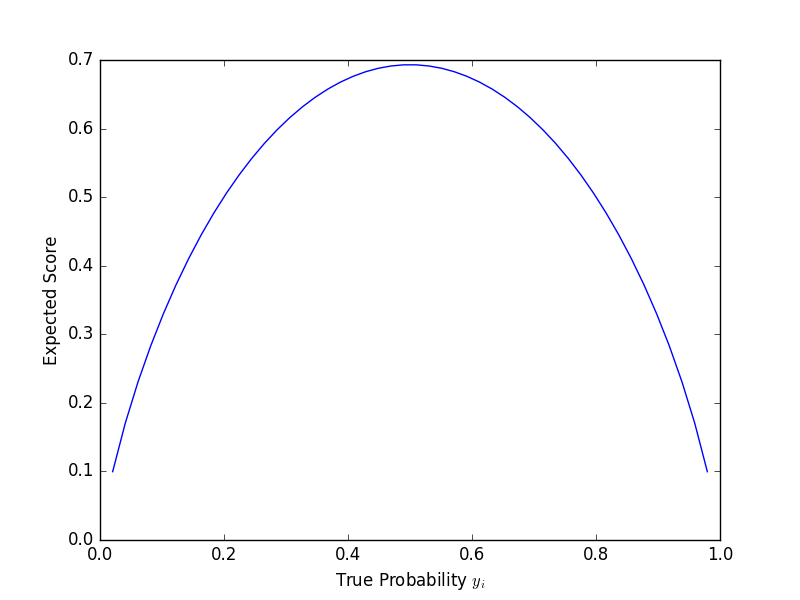
\includegraphics[scale=0.46]{expected_score}
\centering
\caption{Performance of a Perfect Knowledge Predictor}\label{Fig:perfm}
\end{figure}

\section{Data Sets}\label{Sec:data_set}
Kaggle provides almost three decades' data about NCAA basketball matches, including matches during the regular seasons as well as the tournaments. The data sets are summarised in Table~\ref{Ta:data_set}.
\begin{table}[h!]
\centering
\resizebox{\columnwidth}{!}{
\begin{tabular}{ | l | l | }
\hline
\textbf{Data Set} & \textbf{Description} \\ \hline
RegularSeasonCompactResults & Game-by-game results during regular seasons from 1985-2015\\ \hline
RegularSeasonDetailedResults & More detailed results during regular seasons from 2003-2015  \\ \hline
Seasons & Different seasons present in the dataset\\ \hline
Teams & Different college teams present in the dataset  \\ \hline
TourneyCompactResults & Game-by-game tournament results from 1985-2015 \\ \hline
TourneyDetailedResults & More detailed tournament results from 2003-2015.  \\ \hline
TourneySeeds & The seeds for all teams in a tournament  \\ \hline
TourneySlots & The pair-ups between two teams based on their seeds  \\ \hline
\end{tabular}}
\caption{A Summary of the Data Sets}\label{Ta:data_set}
\end{table}

However, not all data sets are useful. Only two of them are used in this project, namely \textbf{RegularSeasonCompactResults} and \textbf{Teams}. 

\section{Role Assignment}
Table~\ref{Ta:role_assgn} shows the assignment of roles for each team member in this project. 
\begin{table}[h!]
\centering
\resizebox{\columnwidth}{!}{
\begin{tabular}{ | l | l | l | }
\hline
\textbf{Team member} & \textbf{Role} & \textbf{Responsibility} \\ \hline
Joe Tan Chin Yong & Data Scientist & To build predictive models \\ \hline
Liu Zeyan & Data Analyst & To optimise selected models \\ \hline
Wei Yumou & Data Scientist & To build predictive models \\ \hline
Xie Dai & Statistician & To provide mathematical knowledge  \\ \hline
\end{tabular}}
\caption{Role Assignment}\label{Ta:role_assgn}
\end{table}


%2.0 DATASET
%
%We use three datasets in this project:
%
%2.1 RegularSeasonDetailedResults.csv
%
%This file identifies the game-by- game results for 13 seasons of historical data, from 2003 to 2015. Each year, it includes all games played from daynum 0 through 132.
%
%Each row in the file represents a single game played. It includes team-level total statistics for each game. We use the data from 2013 to 2015 as only the recent data is relevant to our prediction.
